%%%%%%%%%%%%%%%%%%%%%%%%%%%%%%%%%%%%%%%%%%%%%%%%%%%%%%%%%%%%%%%%%%%%%%
% How to use writeLaTeX: 
%
% You edit the source code here on the left, and the preview on the
% right shows you the result within a few seconds.
%
% Bookmark this page and share the URL with your co-authors. They can
% edit at the same time!
%
% You can upload figures, bibliographies, custom classes and
% styles using the files menu.
%
%%%%%%%%%%%%%%%%%%%%%%%%%%%%%%%%%%%%%%%%%%%%%%%%%%%%%%%%%%%%%%%%%%%%%%

\documentclass[12pt]{article}
\usepackage{sbc-template}
\usepackage{graphicx,url}
\usepackage[brazil]{babel}   
\usepackage[utf8]{inputenc} 
\usepackage{float}

     
\sloppy

\title{Trabalho Prático - Processamento e Análise de Imagens}

\author{Felipe Costa Amaral, Henrique Mendonça Castelar Campos, Larissa Kaweski Siqueira}

\begin{document} 

\maketitle

     
\begin{abstract} 
This article proposes and implements an interface capable of loading images and classifying them as containing or not cancer cells. Two artificial intelligences will be implemented capable of classifying between five types of cancers and the healthy cell.
Besides this classifier, the interface will be capable of processing and analyzing the image.
\end{abstract}
     
\begin{resumo} 
Este artigo propõe e implementa uma interface capaz de ler imagens e classificá-las como contendo ou não células cancerígenas. Serão implementadas 2 inteligências artificiais capazes de classificar entre 5 tipos de câncer e a célula saudável.
Além deste classificador, a interface será capaz de fazer certos processamentos e análises na imagem.
\end{resumo}

\section{Introdução}

\paragraph{}O Câncer Cervical, também conhecido como Câncer de Colo de Útero, é uma doença comum entre as mulheres ao redor do mundo. Um dos mecanismos utilizados para a prevenção desse tipo de doença é o uso de imagens médicas para diagnóstico. Um dos métodos de imagem médica utilizados é a citologia, por meio do exame Papanicolau, que detecta anomalias celulares. Ele consiste na extração de amostras de células do paciente, e a aplicação de corantes nelas. Dependendo da forma como as células reagem aos corantes, isso indica a presença ou não de câncer.

\paragraph{}Este artigo aborda o desenvolvimento de técnicas de aprendizado de máquina para a detecção de células cancerosas no exame Papanicolau, por meio de dois classificadores: o \textit{Support Vector Machines} (SVM) e o \textit{Residual Neural Network} de 50 camadas (ResNet50).

\section{Implementação}

\paragraph{}A implementação da solução de software foi feita na linguagem de programação Python. Para isso foram criados três pacotes (packages): modelo, visão e controlador, seguindo o padrão Model View Controller.

\paragraph{}No pacote modelo foram criadas as classes:

\begin{itemize}
    \item \textit{ImagemRGB}, que implementa os métodos e atributos utilizados para a manipulação de uma imagem RGB.
    
    \item \textit{ImagemHSV}, que implementa os métodos e atributos utilizados para a manipulação de uma imagem HSV.
    
    \item \textit{ImagemTonsCinza}, que implementa os métodos e atributos utilizados para a manipulação de uma imagem em tons de cinza.
    
    \item \textit{Imagem}, classe abstrata que é herdada pelas demais classes de Imagem, que implementa os métodos e atributos comuns utilizados na manipulação de imagens.
\end{itemize}

\paragraph{}No pacote visão (visao) foram criadas as classes:

\begin{itemize}
    \item \textit{FrameImagem}, que é o frame que é exibido quando uma imagem é mostrada.

    \item \textit{FramePrincipal}, que é o primeiro frame a ser mostrado ao abrir o programa.
    
    \item \textit{FrameClassificador}, que mostra as opções para classificar a imagem.
    
    \item \textit{FrameDescritoresHaralick}, que mostra os Descritores de Haralick.

    \item \textit{FrameMomentosInvariantesHu}, que mostra os Momentos Invariantes de Hu.

    \item \textit{JanelaPrincipal}, que é responsável por mostrar a janela principal do programa.
    
    \item \textit{JanelaZoom}, que mostra opções avançadas de zoom na imagem.
\end{itemize}

\paragraph{}No pacote controlador foi criada a classe Controlador, que é responsável por relacionar a interface gráfica com os dados do modelo.

\paragraph{}A interface gráfica foi construída com o uso da biblioteca tkinter, nativa do Python. Para isso foram criadas duas janelas e cinco frames.

\paragraph{}As janelas desenvolvidas foram:

\begin{itemize}
    \item A janela principal, que é a primeira janela aberta pelo programa.

    \item A janela de zoom, que permite a especificação da nova área da imagem a ser exibida.
\end{itemize}

\paragraph{}E os frames desenvolvidos foram:

\begin{itemize}
    \item Frame principal, que é o primeiro frame a ser exibido pelo programa. Nele contém os nomes dos desenvolvedores.

    \item Frame imagem, que é o frame utilizado na exibição de imagens.

    \item Frame classificador, que é o frame utilizado para classificar uma imagem.

    \item Frame descritores de Haralick, que mostra os Descritores de Haralick.

    \item Frame momentos invariantes de Hu, que mostra os Momentos invariantes de Hu.
\end{itemize}

\begin{figure}
    \centering
    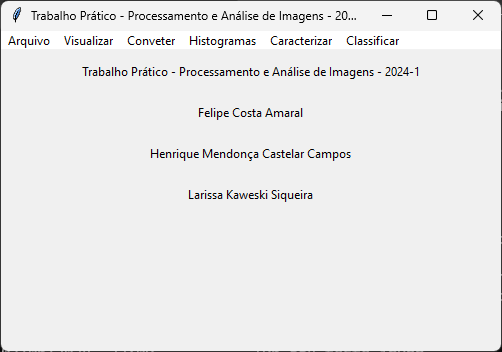
\includegraphics{Captura de tela 2024-06-10 094756.png}
    \caption{Janela principal, quando o programa é iniciado.}
    \label{fig:janela-principal}
\end{figure}

\paragraph{}Na janela principal é mostrado a barra de menu com os menus: ‘Arquivo’, ‘Visualizar’, ‘Converter’, ‘Histogramas’, ‘Caracterizar’ e ‘Classificar’.

\paragraph{}O menu ‘Arquivo’ possui o botão ‘Abrir imagem’, que permite abrir um arquivo de imagem.

\paragraph{}O menu ‘Visualizar’ possui os botões:

\begin{itemize}
    \item ‘Aumentar zoom (Simples)’, que permite aumentar o zoom da imagem no seu centro.

    \item ‘Aumentar zoom (Avançado)’, que permite aumentar o zoom por meio da inserção da nova fronteira.

    \item ‘Remover zoom’, que permite retirar o zoom.
\end{itemize}

\paragraph{}O menu ‘Converter’ possui os botões:

\begin{itemize}
    \item ‘RGB’, que converte a imagem para RGB.
    
    \item ‘Tons de cinza’, que converte a imagem para tons de cinza.
    
    \item ‘HSV’, que converte a imagem para HSV.
\end{itemize}

\paragraph{}O menu ‘Histogramas’ possui os botões:

\begin{itemize}
    \item ‘Tons de cinza’, que gera e mostra o histograma da imagem em tons de cinza.

    \item 'HSV\_2D', que gera e mostra o histograma HSV 2D, relacionando os valores de Hue com Value.

    \item Submenu ‘HSV’, que gera e mostra os histogramas para ‘Hue’, ‘Saturation’ e ‘Value’.
\end{itemize}

\paragraph{}O menu ‘Caracterizar’ possui os botões:

\begin{itemize}
    \item ‘Descritores de Haralick’, que mostra os Descritores de Haralick.

    \item ‘Momentos invariantes de Hu’, que mostra os Momentos invariantes de Hu.
\end{itemize}

\paragraph{}E o botão ‘Classificar’, que alterna para o frame de classificação, que mostra as opções para classificar a imagem.

\begin{figure}
    \centering
    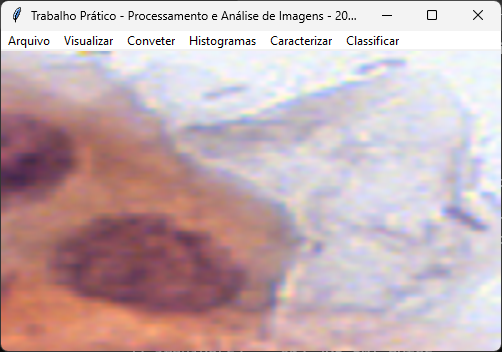
\includegraphics{Captura de tela 2024-06-10 094827.png}
    \caption{Janela principal, quando uma imagem é aberta.}
    \label{fig:janela-principal-imagem-aberta}
\end{figure}

\begin{figure}
    \centering
    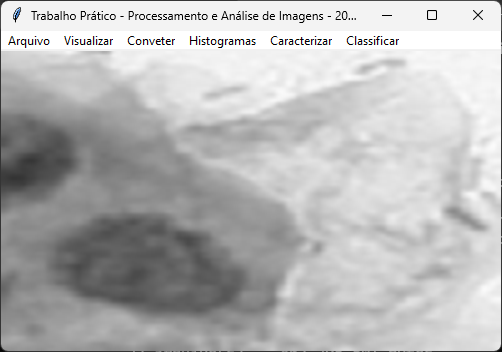
\includegraphics{Captura de tela 2024-06-10 094843.png}
    \caption{Janela principal, exibindo uma imagem em tons de cinza.}
    \label{fig:janela-principal-tons-cinza}
\end{figure}

\begin{figure}
    \centering
    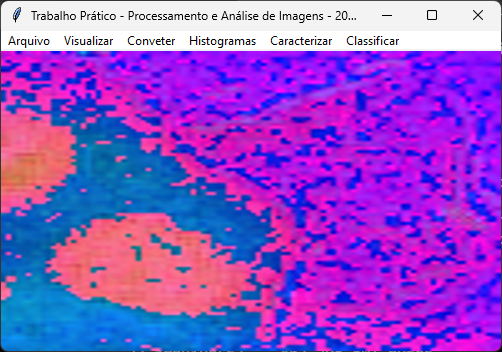
\includegraphics{Captura de tela 2024-06-10 094858.png}
    \caption{Janela principal, exibindo uma imagem HSV.}
    \label{fig:janela-principal-hsv}
\end{figure}

\begin{figure}
    \centering
    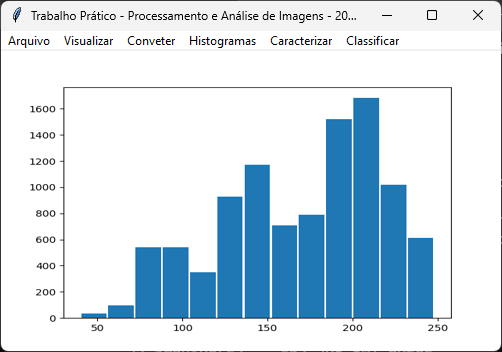
\includegraphics{Captura de tela 2024-06-10 094919.png}
    \caption{Janela principal, exibindo o histograma de uma imagem em tons de cinza.}
    \label{fig:janela-principal-histograma-tons-cinza}
\end{figure}

\begin{figure}
    \centering
    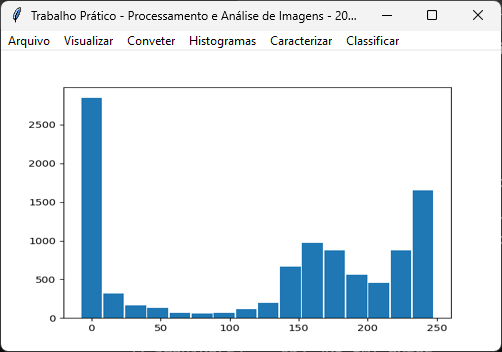
\includegraphics{Captura de tela 2024-06-10 094944.png}
    \caption{Janela principal, exibindo o histograma Hue da imagem HSV.}
    \label{fig:janela-principal-histograma-hue}
\end{figure}

\begin{figure}
    \centering
    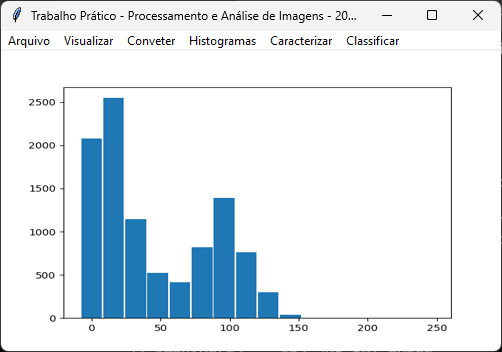
\includegraphics{Captura de tela 2024-06-10 095002.png}
    \caption{Janela principal, exibindo o histograma Saturation da imagem HSV.}
    \label{fig:janela-principal-histograma-saturation}
\end{figure}

\begin{figure}
    \centering
    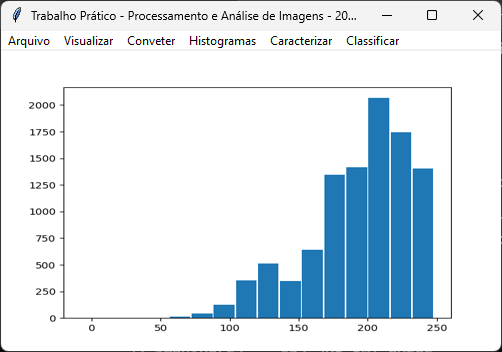
\includegraphics{Captura de tela 2024-06-10 095102.png}
    \caption{Janela principal, exibindo o histograma Value da imagem HSV.}
    \label{fig:janela-principal-histograma-value}
\end{figure}

\begin{figure}
    \centering
    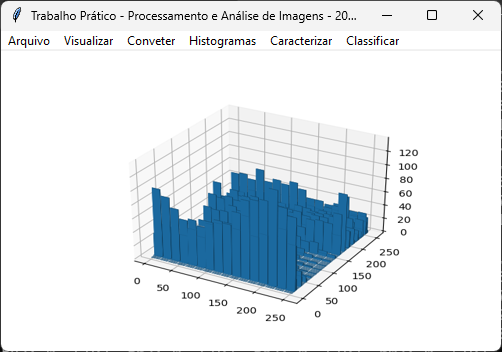
\includegraphics{Captura de tela 2024-06-10 095121.png}
    \caption{Janela principal, exibindo o histograma 2D da imagem HSV.}
    \label{fig:janela-principal-histograma-2d-hsv}
\end{figure}

\begin{figure}
    \centering
    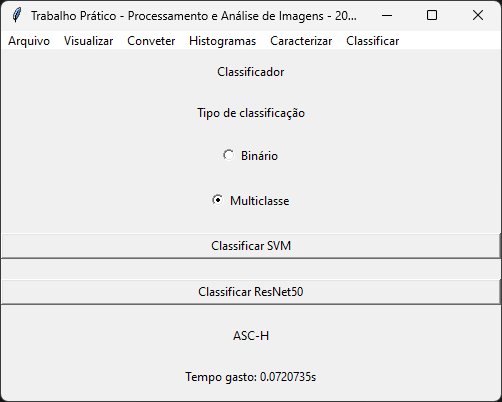
\includegraphics{Captura de tela 2024-06-16 120712.png}
    \caption{Janela principal, exibindo as opções para classificar a imagem.}
    \label{fig:janela-principal-classificar-imagem}
\end{figure}

\begin{figure}
    \centering
    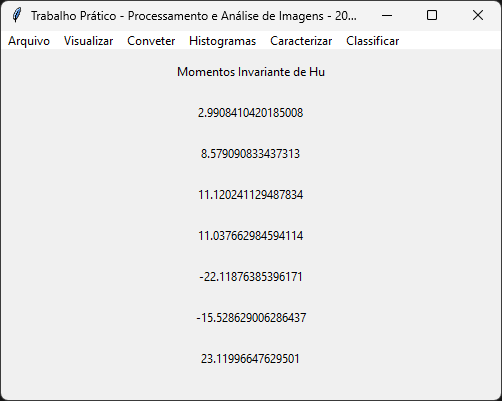
\includegraphics{Captura de tela 2024-06-16 215855.png}
    \caption{Janela principal, mostrando os Momentos Invariantes de Hu.}
    \label{fig:janela-principal-momentos-invariante-hu}
\end{figure}

\begin{figure}
    \centering
    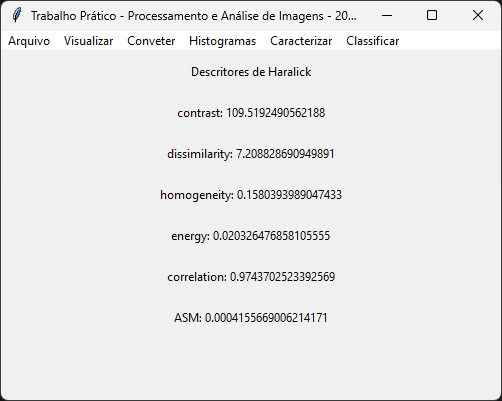
\includegraphics{Captura de tela 2024-06-16 215907.png}
    \caption{Janela principal, mostrando os Descritores de Haralick.}
    \label{fig:janela-principal-descritores-haralick}
\end{figure}

\paragraph{}As bibliotecas utilizadas junto ao programa foram:

\begin{itemize}
    \item Numpy, que é utilizado para a manipulação de vetores.
    
    \item Pillow, que é utilizado para o carregamento e manipulação de imagens.
    
    \item TensorFlow, que é utilizado para a criação dos modelos de aprendizado de máquina (SVM e ResNet50).

    \item Matplotlib, que é utilizado para a geração de gráficos (nos histogramas).
\end{itemize}

\section{Resultados}

\subsection{Qualidade dos resultados}

\begin{figure}
    \centering
    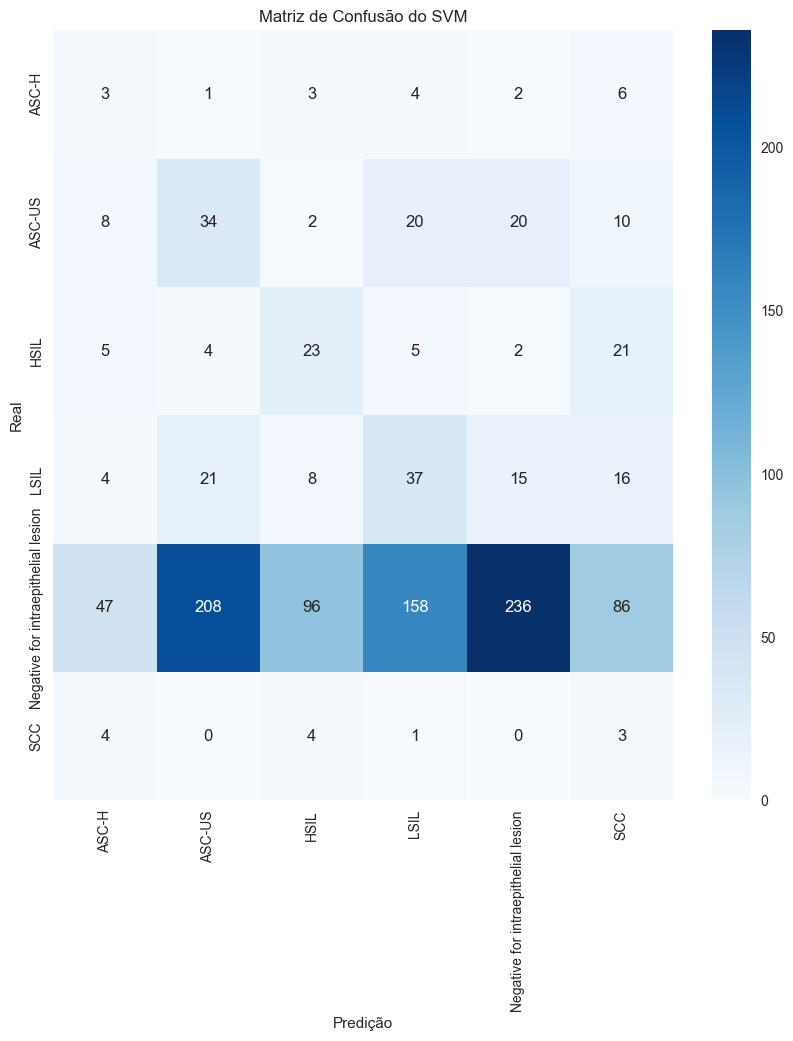
\includegraphics[width=\textwidth]{Matriz confusao SVM.png}
    \caption{Matriz de confusão do SVM}
    \label{fig:matriz-confusao-svm}
\end{figure}

\begin{table}[]
    \centering
    \begin{tabular}{|c|c|}
        \hline
         Métrica & Valor\\
         \hline
         Taxa de Verdadeiro Positivo & 0,46149403734347655\\
         \hline
         Taxa de Verdadeiro Negativo & 0,865422535324905\\
         \hline
         Taxa de Falso Positivo & 0,13457746467509502\\
         \hline
         Taxa de Falso Negativo & 0,5385059626565234\\
         \hline
         Precisão & 0,2630684113588874\\
         \hline
         Sensibilidade & 0,46149403734347655\\
         \hline
         Acurácia & 0,7842680523203728\\
         \hline
         F-Measure & 0,2559065269629602\\
         \hline
    \end{tabular}
    \caption{Métricas do SVM.}
    \label{tab:metricas-svm}
\end{table}

\begin{figure}
    \centering
    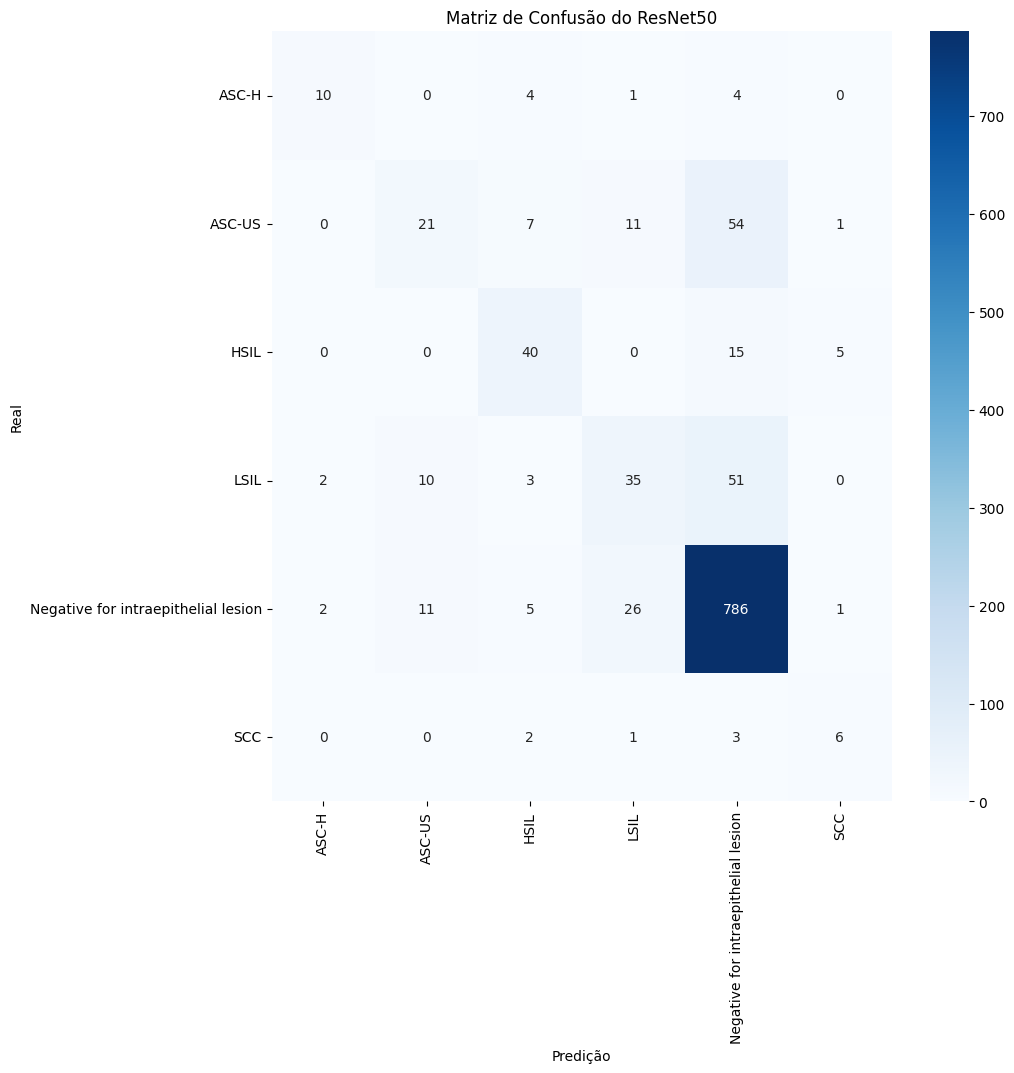
\includegraphics[width=\textwidth]{Matriz confusao ResNet50.png}
    \caption{Matriz de confusão do ResNet50}
    \label{fig:matrix-confusao-resnet50}
\end{figure}

\begin{table}[]
    \centering
    \begin{tabular}{|c|c|}
        \hline
         Métrica & Valor\\
         \hline
         Taxa de Verdadeiro Positivo & 0,8993029942974969\\
         \hline
         Taxa de Verdadeiro Negativo & 0,9807208072160782\\
         \hline
         Taxa de Falso Positivo & 0,019279192783921716\\
         \hline
         Taxa de Falso Negativo & 0,10069700570250299\\
         \hline
         Precisão & 0,9328230136088257\\
         \hline
         Sensibilidade & 0,8993029942974969\\
         \hline
         Acurácia & 0,9865018216568119\\
         \hline
         F-Measure & 0,9149068540667632\\
         \hline
    \end{tabular}
    \caption{Métricas do ResNet50.}
    \label{tab:metricas-resnet50}
\end{table}

\paragraph{}O ResNet50 mostrou um resultado melhor que o SVM, porém as métricas relevantes não foram alcançadas com a precisão desejada. Esse desempenho era esperado pois as máquinas utilizadas para treinar o modelo não tinham as configurações ideais para esse tipo de computação.

\paragraph{}Através da matriz de confusão do modelo SVM, foi possível concluir que o Supporting Vector Machine não é adequado para a identificação de células cancerígenas.

\paragraph{}O SVM foi treinado de diversas formas diferentes, sempre maximizando o score em um valor fixo, o que significa que houve overfit durante o treinamento.

\paragraph{}Novamente houve a tentativa de treinamento balanceando a base de treinamento porém a solução não foi eficiente o suficiente para ser satisfatória.
Entretanto foi possível evitar o overfit e garantir que o resultado era melhor do que aleatório.

\subsection{Tempo}

\begin{figure}
    \centering
    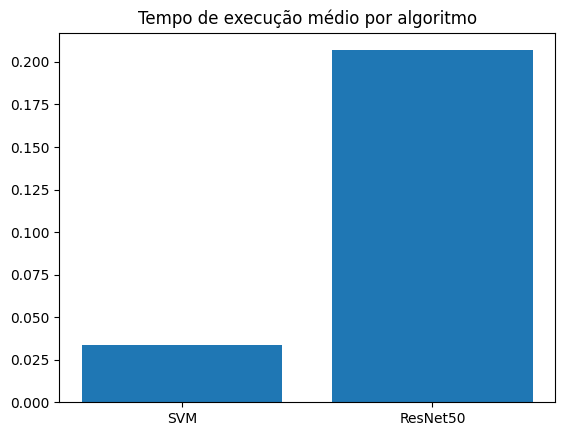
\includegraphics{ResNet50 vs SVM media.png}
    \caption{Gráfico comparando o tempo gasto médio de classificação no SVM e no ResNet50.}
    \label{fig:grafico-svm-vs-resnet-tempo}
\end{figure}

\paragraph{}Através do tempo médio de processamento dos modelos, foi possível concluir que o Supporting Vector Machines é mais rápido para classificar uma única imagem que o Residual Neural Network de 50 camadas.

\begin{figure}[H]
    \centering
    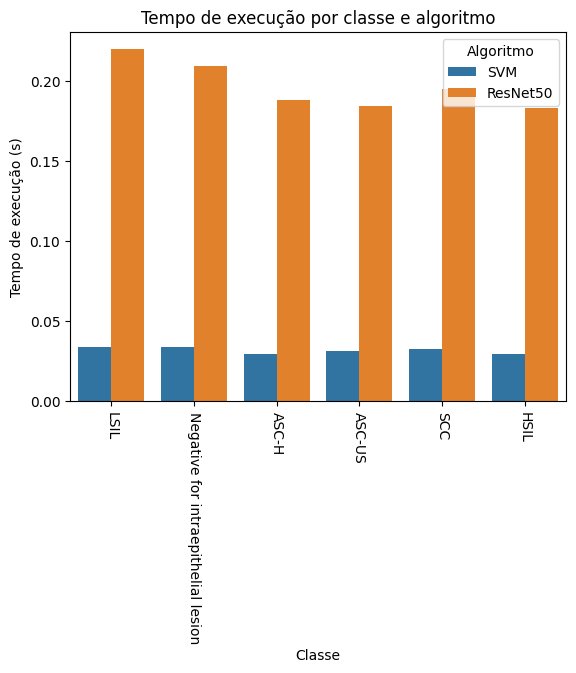
\includegraphics{ResNet50 vs SVM por classe.png}
    \caption{Gráfico comparando o tempo gasto de classificação no SVM e no ResNet50 por classe.}
    \label{fig:grafico-svm-vs-resnet-tempo-por-classe}
\end{figure}

\paragraph{}Não houve diferença de tempo significativa na classificação entre elementos de classe diferentes.

\section{Conclusão}
\paragraph{}O presente trabalho apresentou o desenvolvimento de uma interface para classificação de imagens de células cancerígenas utilizando dois modelos de aprendizado de máquina: Support Vector Machines (SVM) e Residual Neural Network de 50 camadas (ResNet50). Através da implementação e análise dos resultados, foi possível verificar que o modelo ResNet50 obteve desempenho significativamente superior em comparação ao SVM, com melhores métricas de precisão, sensibilidade e acurácia.

\paragraph{}Os resultados mostraram que, enquanto o SVM apresentou problemas de overfitting e uma taxa de verdadeiro positivo inferior a 50\%, o ResNet50 demonstrou uma alta taxa de verdadeiro positivo e um baixo índice de falsos negativos. Contudo, apesar da superioridade do ResNet50, ambos os modelos não alcançaram a precisão desejada, indicando a necessidade de ajustes e melhorias no processo de treinamento e otimização dos modelos.

\paragraph{}Além das análises de desempenho, a implementação destacou a importância da escolha adequada dos modelos de aprendizado de máquina e da infraestrutura computacional necessária para o treinamento eficiente desses modelos. O tempo de processamento também foi um fator relevante, com o SVM se mostrando mais rápido na classificação de imagens individuais, enquanto o ResNet50, apesar de mais lento, apresentou resultados mais robustos.

\paragraph{}Portanto, conclui-se que a utilização de redes neurais profundas como o ResNet50 é mais adequada para a tarefa de classificação de células cancerígenas, desde que sejam realizados aprimoramentos no treinamento e na otimização do modelo. Este trabalho contribui para o avanço das técnicas de diagnóstico automatizado, proporcionando uma base para futuras pesquisas e desenvolvimento de soluções mais eficazes na área de processamento e análise de imagens médicas.

\paragraph{}

\nocite{cancerCervical}
\nocite{coloracaoPapanicolau}
\nocite{papanicolauStain}
\nocite{resnet}
\nocite{svm}

\bibliographystyle{sbc}
\bibliography{bibliografia}


\end{document}
